% Data flow: datasets to evaluation
\documentclass[tikz,border=5pt]{standalone}
\usetikzlibrary{arrows.meta,shapes.geometric}
\begin{document}
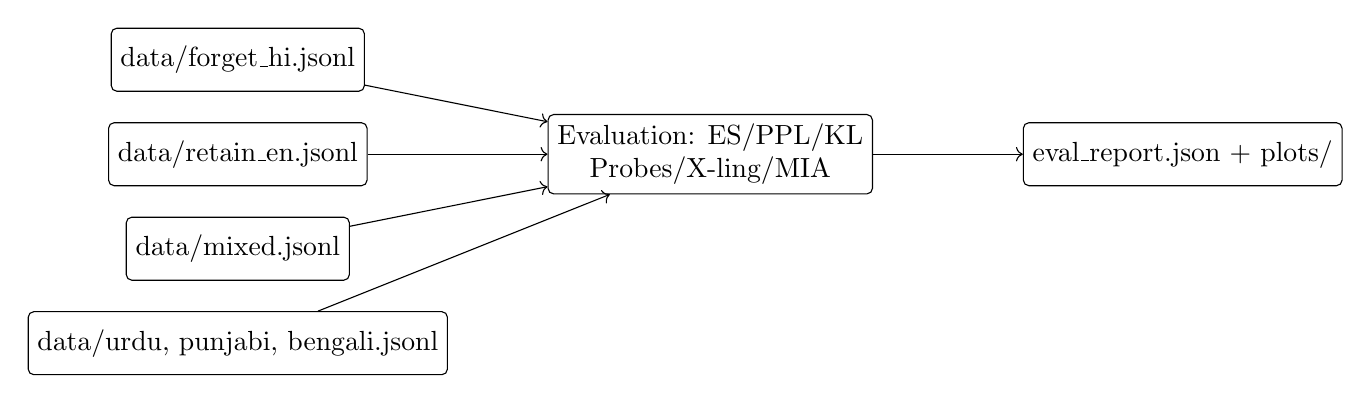
\begin{tikzpicture}[
  node distance=10mm and 12mm,
  box/.style={draw, rounded corners=2pt, minimum width=28mm, minimum height=8mm, align=center},
  line/.style={->}
]
\node[box] (forget) at (0,0) {data/forget\_hi.jsonl};
\node[box] (retain) at (0,-12mm) {data/retain\_en.jsonl};
\node[box] (mixed)  at (0,-24mm) {data/mixed.jsonl};
\node[box] (xlang)  at (0,-36mm) {data/{urdu, punjabi, bengali}.jsonl};

\node[box] (eval) at (60mm,-12mm) {Evaluation: ES/PPL/KL\\Probes/X‑ling/MIA};
\draw[line] (forget) -- (eval);
\draw[line] (retain) -- (eval);
\draw[line] (mixed) -- (eval);
\draw[line] (xlang) -- (eval);

\node[box] (report) at (120mm,-12mm) {eval\_report.json + plots/};
\draw[line] (eval) -- (report);
\end{tikzpicture}
\end{document}

